\documentclass[a4paper, 12pt]{article}

\usepackage[portuges]{babel}
\usepackage[utf8]{inputenc}
\usepackage{amsmath}
\usepackage{indentfirst}
\usepackage{graphicx}
\usepackage{multicol,lipsum}

\usepackage[hidelinks]{hyperref}   % adiciona links na TOC e nas citações

% Renomeia o título da TOC
\addto\captionsportuges{
  \renewcommand{\contentsname}
    {Sumário}
}

%%%%%%%%%%%%%%%%%%%%%%%%%%%%%%%%%%%%%%%%%%%%%%%%%%%%%%%%%%
% INÍCIO DO DOCUMENTO
%%%%%%%%%%%%%%%%%%%%%%%%%%%%%%%%%%%%%%%%%%%%%%%%%%%%%%%%%%

\begin{document}
%\maketitle

%%%%%%%%%%%%%%%%%%%%%%%%%%%%%%%%%%%%%%%%%%%%%%%%%%%%%%%%%%%
% CAPA
%%%%%%%%%%%%%%%%%%%%%%%%%%%%%%%%%%%%%%%%%%%%%%%%%%%%%%%%%%%
\begin{titlepage}
	\begin{center}
    	\begin{figure}[!ht]
        	\centering
        	
\includegraphics[width=3cm]{./imgs/uffs.png}
    	\end{figure}
    
    	\Huge{Universidade Federal da Fronteira Sul}\\
    	\large{Campus Chapecó}\\ 
    	\large{Bacharelado em Ciência da Computação}\\ 
    	
    	\vspace{15pt}
        \vspace{95pt}
        
        \textbf{\LARGE{Exercícios indicados nas aulas 05 e 06}}\\
    	
        \vspace{3,5cm}
	\end{center}
	
	\begin{flushleft}
	    \begin{tabbing}
			\textbf{Aluno:} Jean Carlo Hilger \\
			\textbf{Professor:} Andrei de Almeida Sampaio Braga \\
        \end{tabbing}
    \end{flushleft}
	
	\vspace{1cm}
	
	\begin{center}
		\vspace{\fill}
		Chapecó, março\\
		2021
	\end{center}
\end{titlepage}


%%%%%%%%%%%%%%%%%%%%%%%%%%%%%%%%%%%%%%%%%%%%%%%%%%%%%%%%%%%
% SUMÁRIO
%%%%%%%%%%%%%%%%%%%%%%%%%%%%%%%%%%%%%%%%%%%%%%%%%%%%%%%%%%%
\newpage
\tableofcontents
\thispagestyle{empty}

\newpage
\pagenumbering{arabic}

%%%%%%%%%%%%%%%%%%%%%%%%%%%%%%%%%%%%%%%%%%%%%%%%%%%%%%%%%%%
% Exercício 1
%%%%%%%%%%%%%%%%%%%%%%%%%%%%%%%%%%%%%%%%%%%%%%%%%%%%%%%%%%%
\newpage
\section*{Exercício 1}
\addcontentsline{toc}{section}{Exercício 1}

Construa um diagrama de estados com 3 estados para um autômato finito
não-determinístico que reconheça a linguagem $\{ w | w$  é uma string de 0’s 1’s
que termina com $00\}$.

\subsection*{Solução 1}
\addcontentsline{toc}{subsection}{Solução 1}

\begin{figure}[!ht]
    \centering
    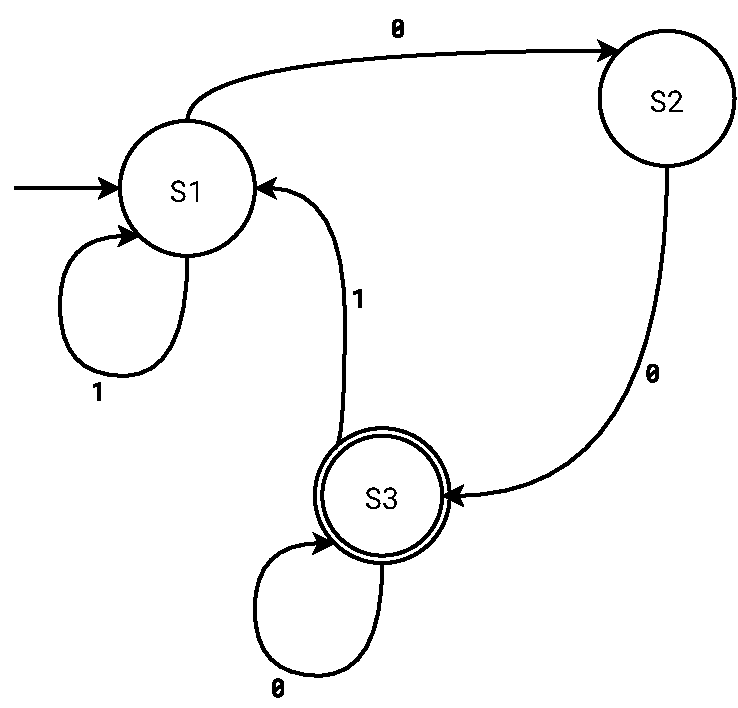
\includegraphics[width=8cm]{./imgs/task-2-1.pdf}
    \caption{Autômato não-determinístico solução}
    \label{fig:solution_t2_1}
\end{figure}


%%%%%%%%%%%%%%%%%%%%%%%%%%%%%%%%%%%%%%%%%%%%%%%%%%%%%%%%%%%
% Exercício 2
%%%%%%%%%%%%%%%%%%%%%%%%%%%%%%%%%%%%%%%%%%%%%%%%%%%%%%%%%%%
\newpage
\section*{Exercício 2}
\addcontentsline{toc}{section}{Exercício 2}

Descreva um autômato finito não-determinístico que reconheça a linguagem
que consiste de toda string do alfabeto $\{0, 1, ..., 9\}$ tal que o último dígito da
string aparece antes na string.

\subsection*{Solução 2}
\addcontentsline{toc}{subsection}{Solução 2}


Inicialmente, imaginemos o mesmo autômato para um alfabeto mais simples, formado apenas por $\{a, b\}$:

\begin{figure}[!ht]
    \centering
    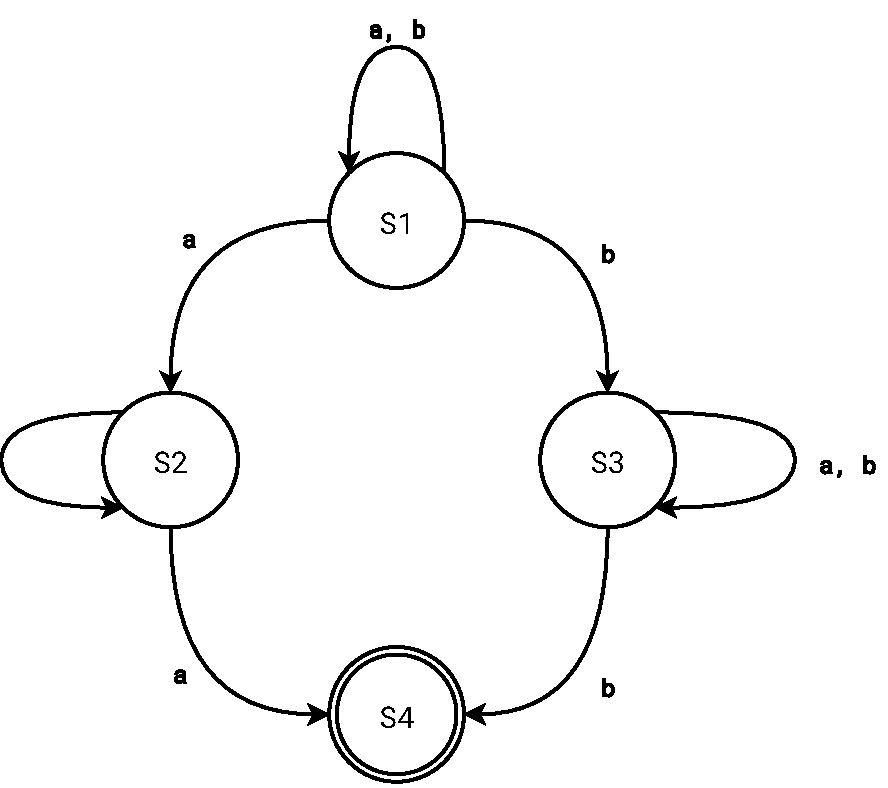
\includegraphics[width=8cm]{./imgs/task-2-2a.pdf}
    \caption{Solução para um caso mais simples.}
    \label{fig:solution_t2_2a}
\end{figure}

Partindo desta ideia podemos descrever um caso geral para um autômato finito 
que aceita toda string de uma linguagem composta por $n$ símbolos, tal que o último
símbolo ocorreu pelo menos uma vez na string:

\begin{figure}[!ht]
    \centering
    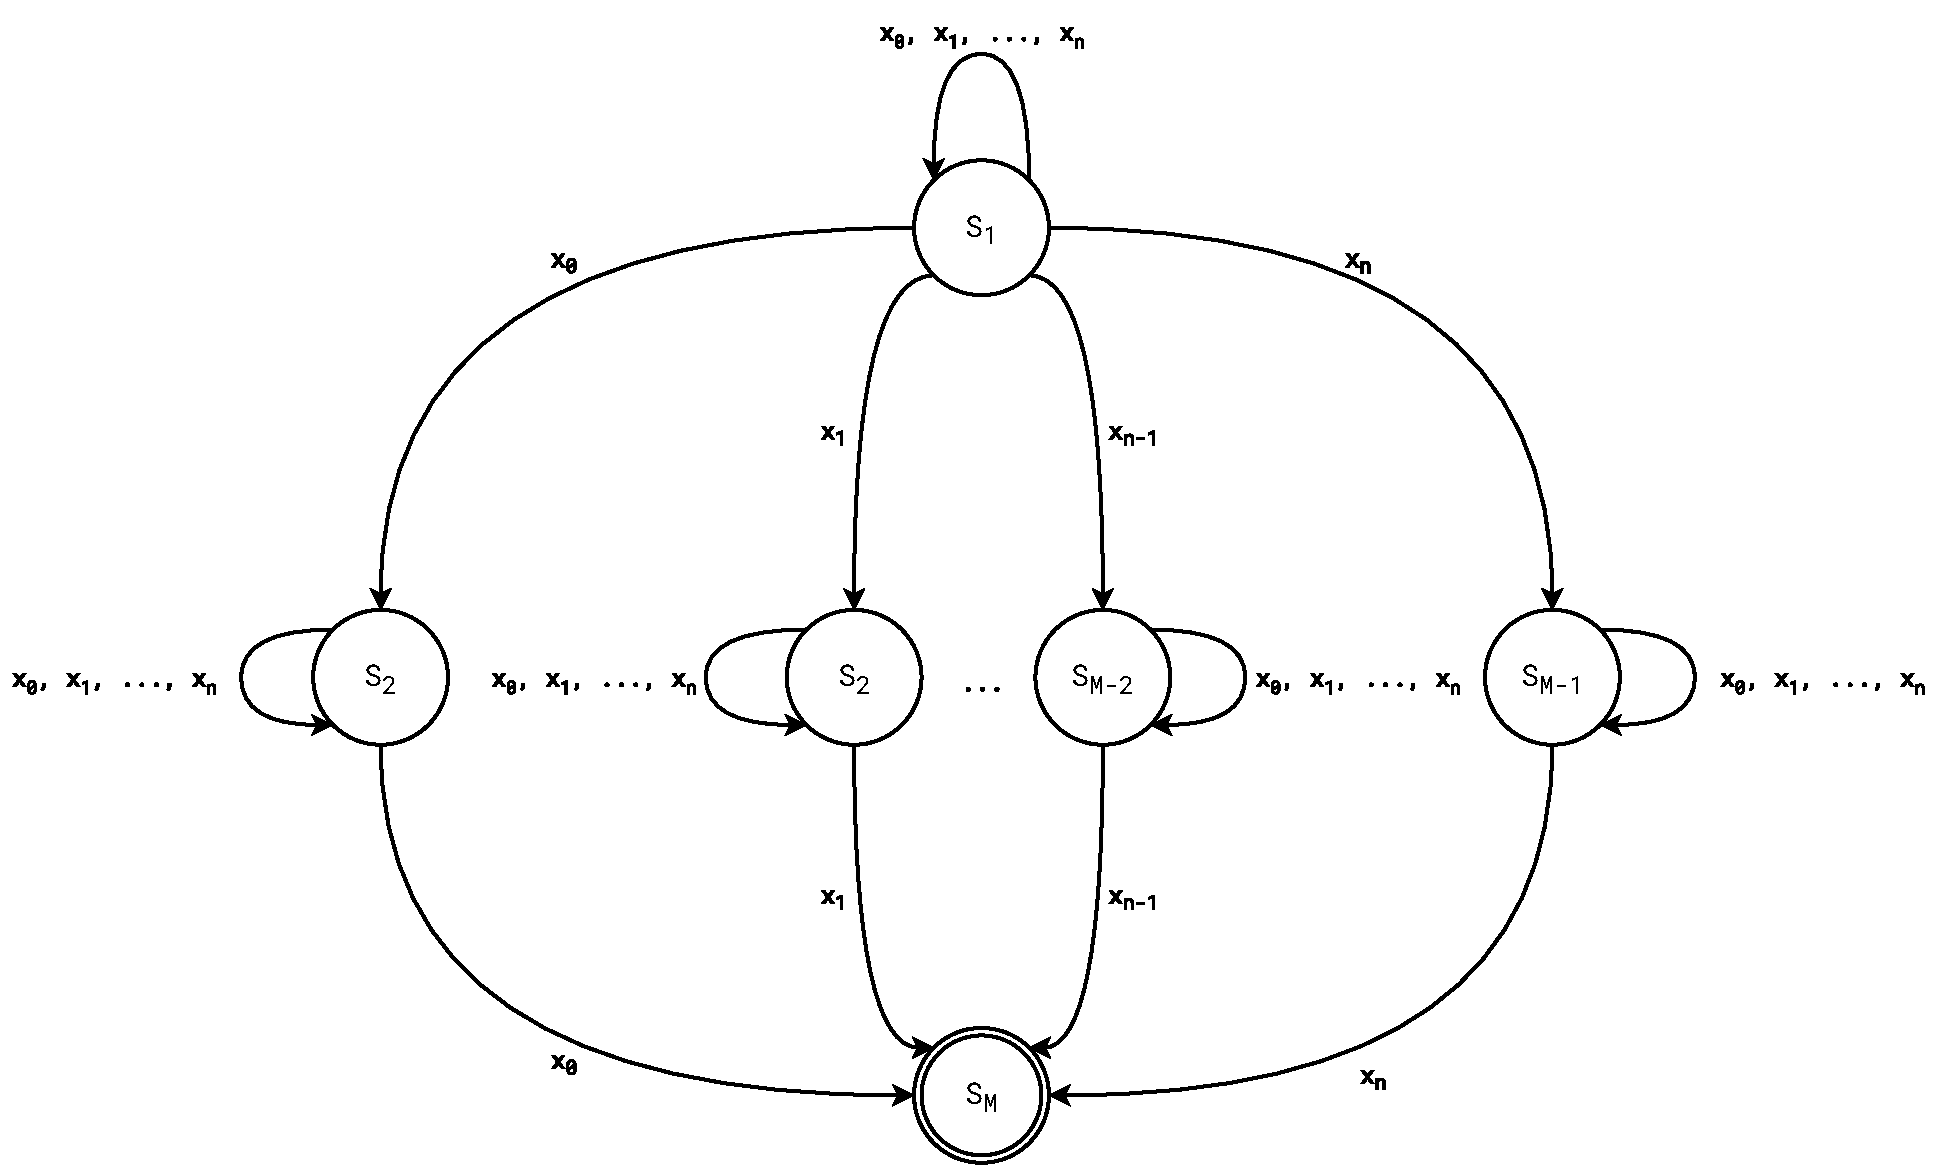
\includegraphics[width=\linewidth]{./imgs/task-2-2b.pdf}
    \caption{Caso geral da solução, para strings de tamanho $n$.}
    \label{fig:solution_t2_2b}
\end{figure}

Assim, a solução dá-se por:

\begin{figure}[!ht]
    \centering
    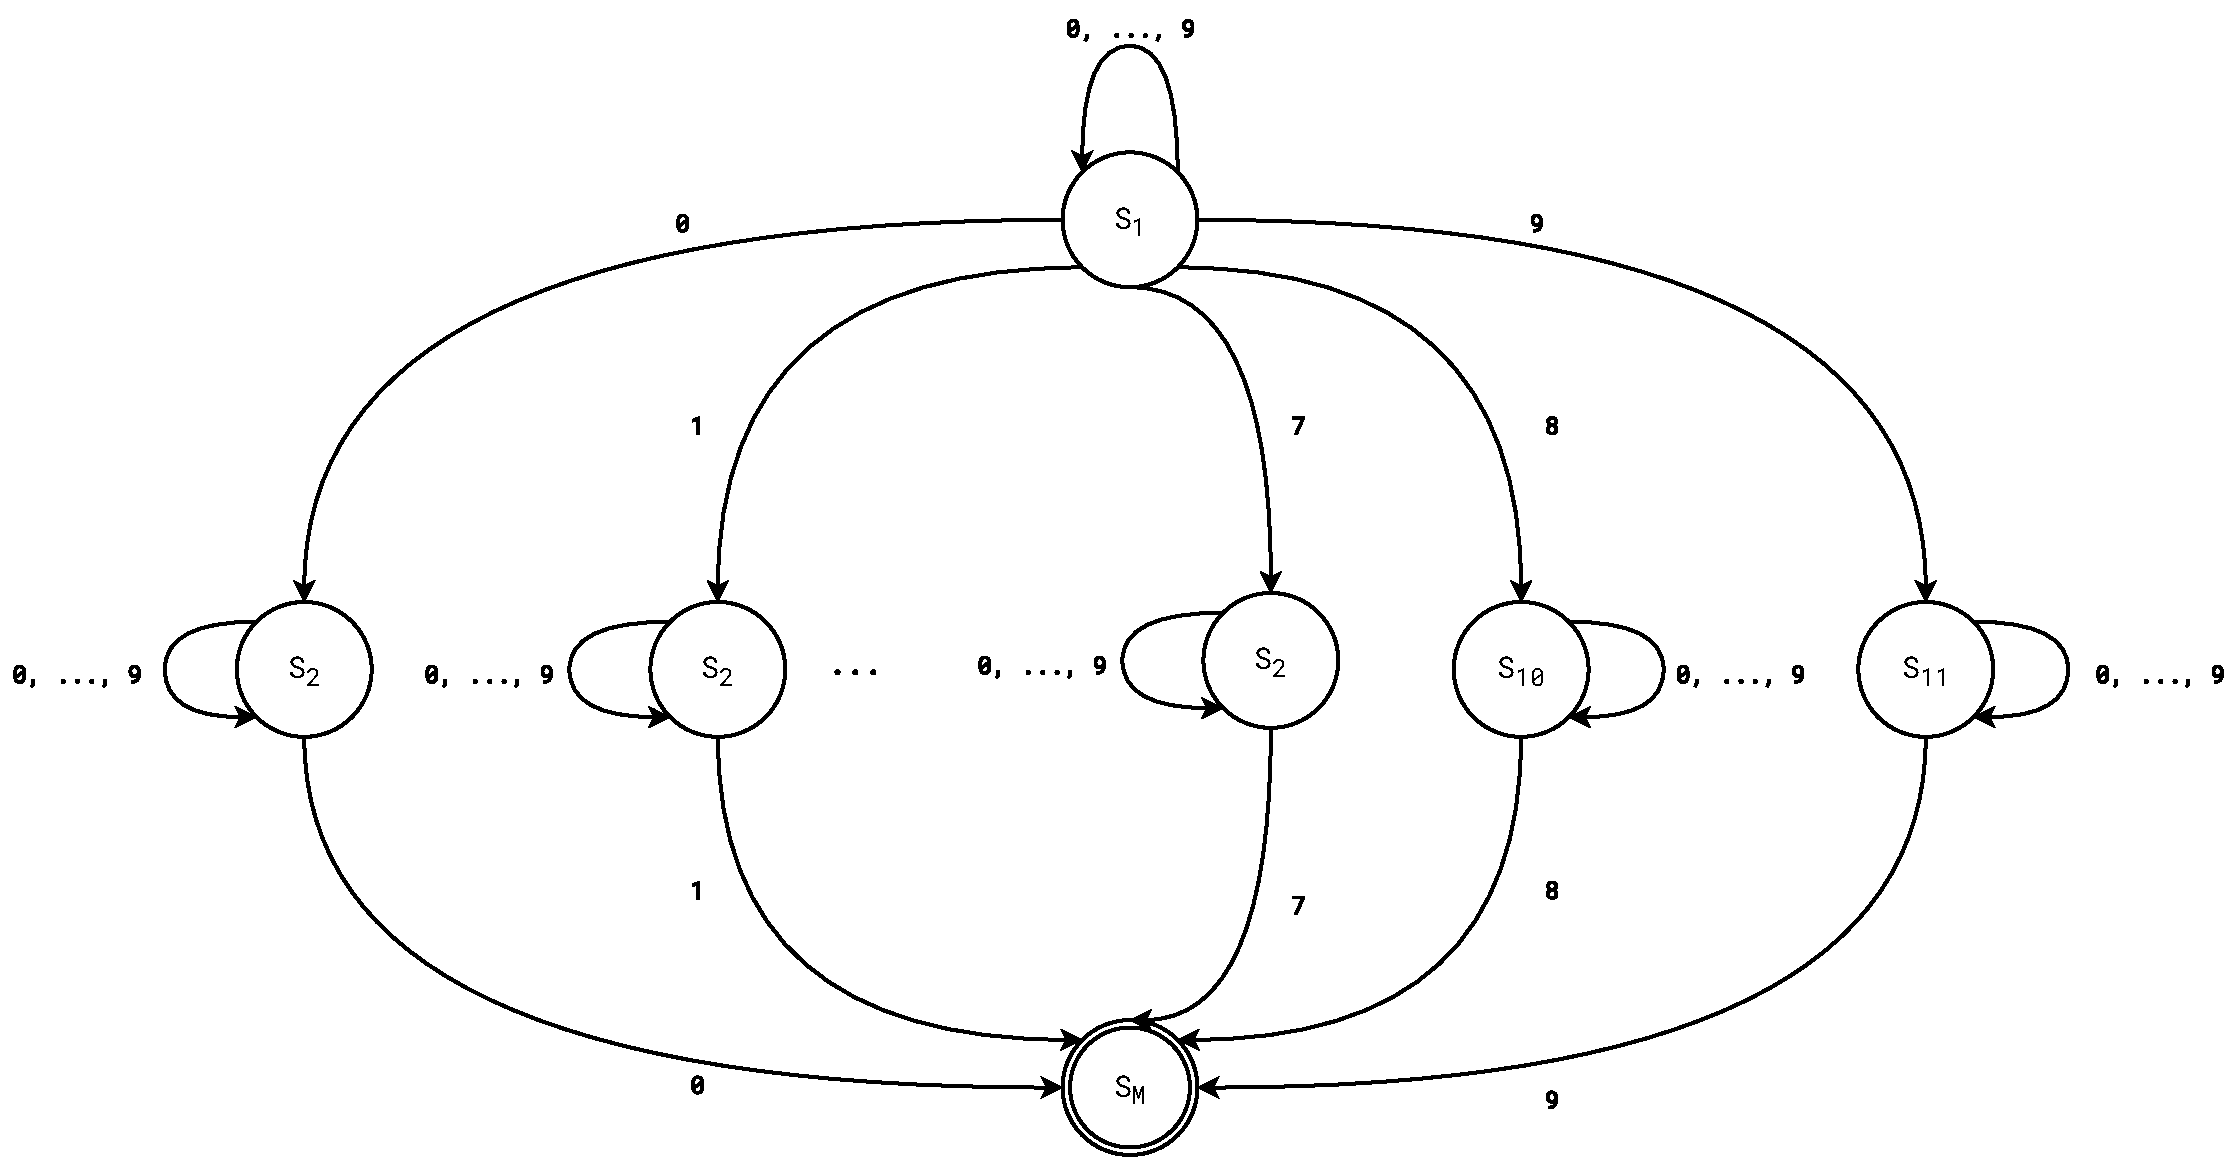
\includegraphics[width=\linewidth]{./imgs/task-2-2c.pdf}
    \caption{Solução para o Exercício 2.}
    \label{fig:solution_t2_2c}
\end{figure}


\end{document}
